\subsubsection{概要}
きなこチームは, 3D-LiDARを用いた自己位置推定の信頼性向上を目的としたシステムを開発した. 
このシステムは自己位置推定にemcl2, 経路計画・走行制御にNav2を採用している. 

開発の背景には、人や車などの動的障害物による自己位置推定の破綻という課題があった。
当初この問題に対し、動的障害物の影響を受けにくい2m以上の高さの点群データのみを使用する手法を採用していた。
また、3Dマップとセンサから得られる点群データは、高さ方向(z軸)の情報を圧縮し2次元平面(xy平面)に投影して処理を行っていた。
しかし、環境の特徴は場所によって異なる高さに存在する。
そのため、この手法では重要な特徴が失われ、自己位置推定が不安定になる問題が発生していた。
この課題を解決するため, ロボットの現在位置に応じて自己位置推定に使用するマップと点群データの高さ範囲を動的に変更できるシステムを新たに開発した. 

\subsubsection{システム構成}
システムの開発のために以下の2つのパッケージを作成した. 

\begin{itemize}
  \item \textbf{map\_manager}
    \begin{itemize}
      \item 複数の2次元マップと高さ範囲のパラメータを管理するパッケージ
      \item ロボットが指定した領域に進入すると, その領域に最適化された2次元マップと高さパラメータを提供
    \end{itemize}
  \item \textbf{pointcloud\_to\_dual\_scan}
    \begin{itemize}
      \item 3D-LiDARの点群データから2種類の2次元スキャンデータを生成
        \begin{itemize}
          \item 障害物回避用のスキャンデータ
          \item 自己位置推定用のスキャンデータ(map\_managerの指定する高さ範囲に基づく)
        \end{itemize}
    \end{itemize}
\end{itemize}

マップデータは, GLIMを用いて事前に3次元マップを作成し, 必要な高さ領域を抽出して2次元の占有格子地図に変換している. 


\subsubsection{システム統合}
図に示すように、3D-LiDARから取得した点群データはpointcloud\_to\_dual\_scanで処理され、2種類の2次元スキャンデータに変換される。
map\_managerは、ロボットの位置に応じて最適な2次元マップと高さパラメータを提供し、emcl2による自己位置推定を安定させる。
Nav2により生成された速度指令値はraspimouseを介してモータードライバに伝達され、ロボットの制御を実現している。

\begin{figure}[h]
  \begin{center}
    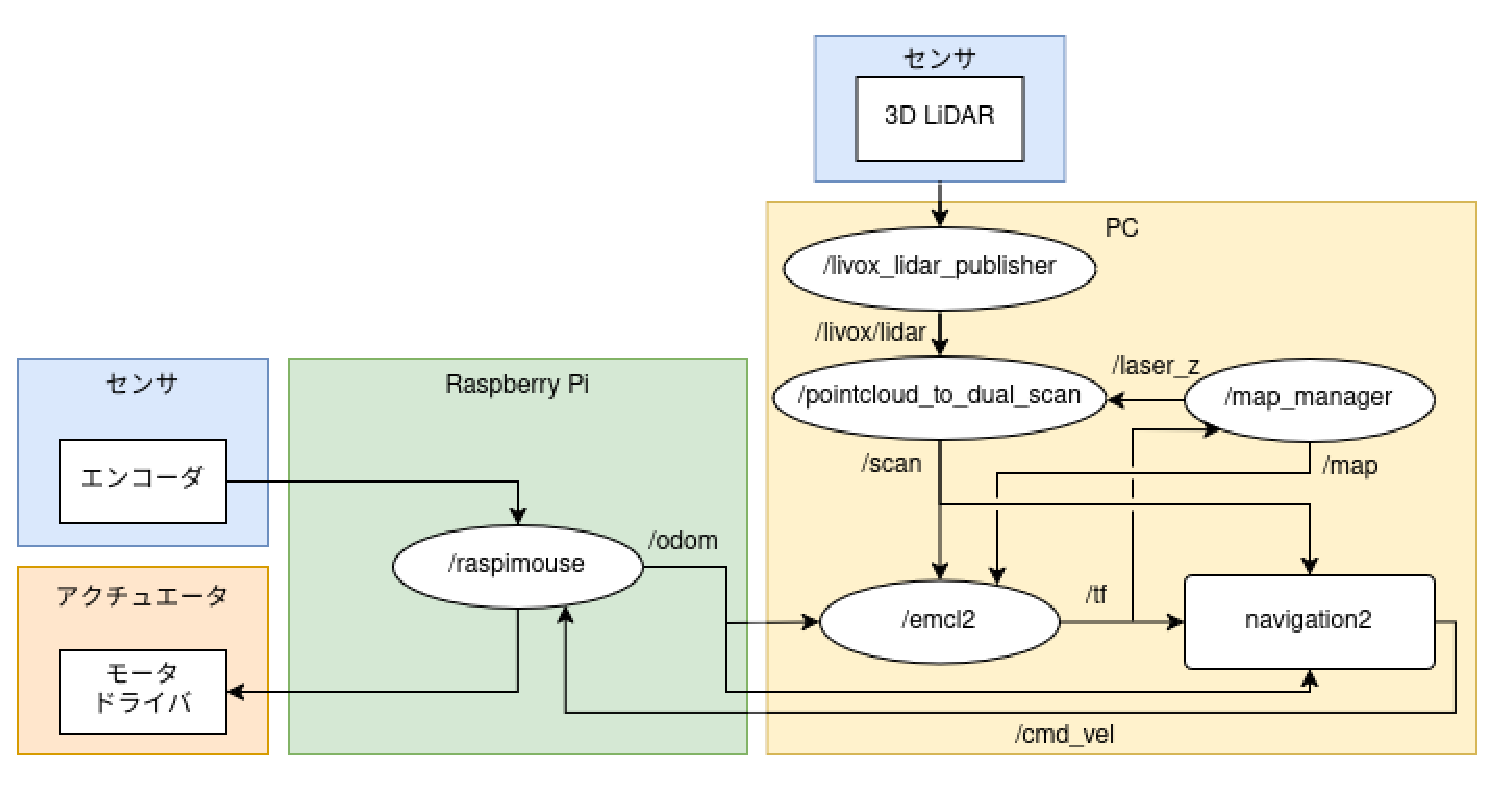
\includegraphics[width=1.0\linewidth]{figs/kinako_system.eps}
    \caption{きなこチームのシステム構成}
    \label{fig:mugimaru_system}
  \end{center}
\end{figure}
